\documentclass[10pt,a4paper]{article}

\usepackage[margin=2.1cm]{geometry}
\usepackage[T1]{fontenc}
\usepackage{newtxtext,newtxmath}
\usepackage{booktabs}
\usepackage{graphicx}
\usepackage{subcaption}
\usepackage{array}
\usepackage{multirow}
\usepackage{amsmath}
\usepackage{xcolor}
\usepackage{tikz}
\usetikzlibrary{positioning,arrows.meta,fit,backgrounds,calc,shapes.geometric}
\usepackage[colorlinks=true,linkcolor=blue!55!black,citecolor=blue!55!black,
            urlcolor=blue!55!black]{hyperref}
\usepackage[numbers,sort&compress]{natbib}
\usepackage{caption}
\captionsetup{font=small,labelfont=bf,width=0.95\linewidth}
\usepackage{titlesec}
\titlespacing*{\section}{0pt}{1.1ex plus .3ex}{0.6ex}
\titlespacing*{\subsection}{0pt}{0.9ex plus .2ex}{0.4ex}

\definecolor{cData}{HTML}{56B4E9}
\definecolor{cAudit}{HTML}{009E73}
\definecolor{cModel}{HTML}{0072B2}
\definecolor{cFuse}{HTML}{E69F00}
\definecolor{cFail}{HTML}{B0B0B0}
\definecolor{cAccent}{HTML}{D55E00}

\newcommand{\auc}{ROC-AUC}
\newcommand{\dlt}[1]{$#1\times10^{-4}$}

\title{\vspace{-1.2cm}\bfseries Where the Gains Come From:\\[2pt]
\large A Controlled Study of Feature, Model-Family and Ensemble Interventions\\
on a 700k-row Synthetic Tabular Benchmark}
\author{The Time Forever \quad (Kaggle: \textsf{adamsmith1112})\\[2pt]
\small Playground Series S6E10 --- Predicting Airline Satisfaction}
\date{October 2026}

\begin{document}
\maketitle

\begin{abstract}
\noindent
Public leaderboards reward the final score, but practitioners rarely know which
interventions actually move it. We study this question on Kaggle Playground S6E10
(699{,}635 training rows, 21 features, \auc{}), where the data are synthesised from a
public airline survey, and we measure every intervention on the same five stratified folds
with paired DeLong inference and record its public-leaderboard effect. An audit of the data
shows why the ceiling is low: 5.66\% of rows share their discrete feature signature with
another row of the opposite label, 48.3\% of the test-time errors are confident errors, and
the generator collapsed the delay distribution (mean 1.18 vs.\ 14.71 minutes), which removes a
signal that exists in the original survey. Single-model work saturates at 0.9605
\auc{}: capacity sweeps and 16 Optuna trials move the score by less than the paired noise
floor of \dlt{2.2}. A ladder of more than twenty interventions then separates what transfers from what does
not. Cross-fitted target statistics of the exact flight distance are the only large single
gain (\dlt{13.5}); afterwards, \emph{new model families} transfer at a rate above one
($+1.0$ \dlt{} cross-validated $\to$ $+1.5$ \dlt{} public), whereas seed averaging
($+0.55 \to +0.1$), ten folds ($+0.14$), five stacking schemes ($\pm 0.3$) and five
feature-side variants do not. The final eight-family logit blend reaches 0.960901
cross-validated and 0.96062 public, i.e.\ rank 1{,}204 of 3{,}061 teams, and we quantify what
the remaining 1.1 \dlt{} to the top decile would cost.
\end{abstract}

\section{Introduction}

Kaggle Playground competitions are a convenient laboratory for tabular machine learning:
the metric is fixed, the data are public, and thousands of teams optimise the same quantity.
They are also a good place to study a question that matters outside competitions:
\emph{which kinds of intervention actually improve generalisation, and which only improve the
number you are looking at?}

We take the October~2026 episode (S6E10, airline passenger satisfaction, binary \auc{}) and run
a controlled study. Every intervention is applied to the same five stratified folds, all
learned transforms are fitted inside the training part of each fold, and every comparison is
reported as a paired difference with a DeLong standard error \citep{delong1988}. The same model
is then submitted to the public leaderboard, so each change has two readings: a cross-validated
one and a leaderboard one.

Our contribution is empirical rather than algorithmic:
\begin{itemize}\itemsep1pt
\item a data audit that explains the low ceiling of the benchmark (label noise, a
      generator artefact in the flight-distance support, a collapsed delay distribution,
      and the semantics of zero-valued ratings);
\item a leakage-safe protocol with paired inference and a pre-registered adoption rule, which
      lets us separate real effects from noise at a resolution of $10^{-4}$;
\item a ladder of more than twenty interventions measured twice (CV and public LB) that yields a
      simple, quantitative rule: \emph{new model families transfer, everything else mostly does
      not};
\item a leaderboard analysis that turns the remaining gap into a cost estimate.
\end{itemize}

\section{Related work}

\paragraph{What wins on tabular data.} Gradient-boosted trees remain the default for
medium-sized tabular problems, and careful benchmarks attribute that to their robustness to
uninformative features and to rotation invariance rather than to any failure of neural
networks \citep{grinsztajn2022,shwartzziv2022}. The neural results improved substantially once
numerical features were embedded rather than standardised \citep{gorishniy2022}, and once
architectures were tuned with a modern recipe \citep{gorishniy2021,holzmuller2024}; parameter
efficient ensembling pushes the same family further \citep{gorishniy2024tabm}. Our ensemble is
built exactly along that axis: we keep LightGBM as the anchor and look for neural members that
are strong \emph{and} decorrelated.

\paragraph{Leakage-safe statistics and paired comparison.} Target encoding of a high-cardinality
key is classical \citep{miccibarreca2001}, and its failure mode --- target leakage inside the
training fold --- is well known; we use the inner cross-fitting that makes the estimate honest.
Comparing two models on the same rows requires a paired test; the DeLong covariance
\citep{delong1988} gives one in closed form, and it is what turns our $10^{-5}$ differences into
statements about noise instead of statements about models. Label noise is usually estimated with
confident learning \citep{northcutt2021}; here the discrete signatures give a direct, model-free
estimate that we can check against the residual errors.

\section{Pipeline and experimental design}
Figure~\ref{fig:pipeline} summarises the study. Data and protocol are fixed first; the
single-model ladder is explored until it saturates; model families are then added and blended;
every candidate is read twice, on the folds and on the public board, and the rejected ideas are
kept in the record because they bound what is worth trying next.

\begin{figure*}[t]
\centering
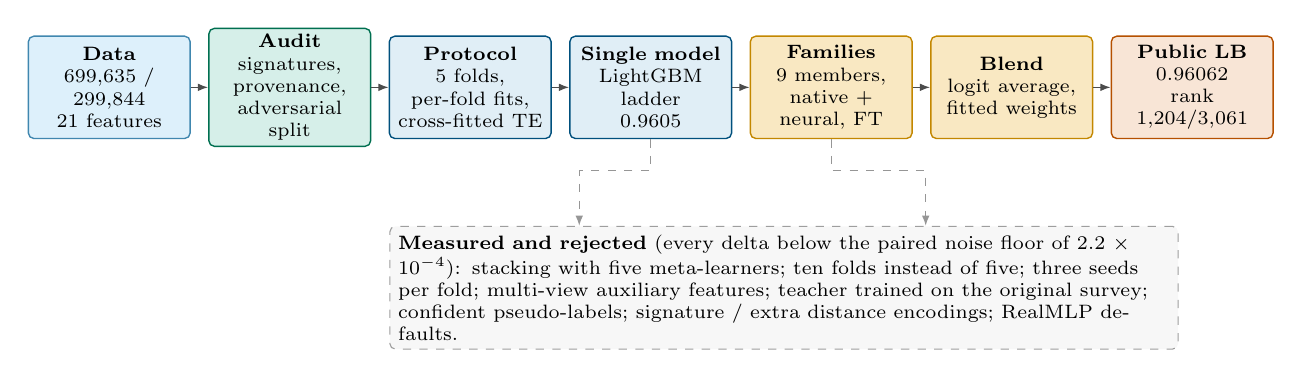
\begin{tikzpicture}[
  font=\scriptsize,
  stage/.style={draw, rounded corners=2pt, align=center, inner sep=2.2pt,
                minimum height=13mm, text width=19mm, line width=0.5pt},
  data/.style={stage, fill=cData!20, draw=cData!75!black},
  audit/.style={stage, fill=cAudit!16, draw=cAudit!70!black},
  model/.style={stage, fill=cModel!12, draw=cModel!70!black},
  fuse/.style={stage, fill=cFuse!24, draw=cFuse!85!black},
  lb/.style={stage, fill=cAccent!16, draw=cAccent!85!black},
  bad/.style={draw=cFail!90!black, dashed, rounded corners=2pt, align=left,
              inner sep=3pt, text width=98mm, fill=cFail!10, font=\scriptsize},
  arr/.style={-{Latex[length=1.3mm]}, line width=0.5pt, draw=black!70},
  badarr/.style={-{Latex[length=1.3mm]}, line width=0.5pt, draw=cFail!85!black, dashed},
]
\node[data] (data) at (0,0) {\textbf{Data}\\699{,}635 / 299{,}844\\21 features};
\node[audit, right=2.2mm of data] (audit) {\textbf{Audit}\\signatures, provenance,\\adversarial split};
\node[model, right=2.2mm of audit] (proto) {\textbf{Protocol}\\5 folds, per-fold fits,\\cross-fitted TE};
\node[model, right=2.2mm of proto] (single) {\textbf{Single model}\\LightGBM ladder\\0.9605};
\node[fuse, right=2.2mm of single] (fams) {\textbf{Families}\\9 members, native +\\neural, FT};
\node[fuse, right=2.2mm of fams] (blend) {\textbf{Blend}\\logit average,\\fitted weights};
\node[lb, right=2.2mm of blend] (lb) {\textbf{Public LB}\\0.96062\\rank 1{,}204/3{,}061};

\draw[arr] (data) -- (audit);
\draw[arr] (audit) -- (proto);
\draw[arr] (proto) -- (single);
\draw[arr] (single) -- (fams);
\draw[arr] (fams) -- (blend);
\draw[arr] (blend) -- (lb);

\node[bad, below=11mm of fams, xshift=-6mm] (rejected)
  {\textbf{Measured and rejected} (every delta below the paired noise floor of \dlt{2.2}):
   stacking with five meta-learners; ten folds instead of five; three seeds per fold;
   multi-view auxiliary features; teacher trained on the original survey; confident
   pseudo-labels; signature / extra distance encodings; RealMLP defaults.};
\draw[badarr] (single.south) -- ++(0,-4mm) -| ([xshift=-26mm]rejected.north);
\draw[badarr] (fams.south) -- ++(0,-4mm) -| ([xshift=18mm]rejected.north);
\end{tikzpicture}
\caption{The study at a glance. The upper chain is the adopted pipeline; the dashed box lists the
interventions that were measured on the same folds and rejected because their effect stayed
inside the noise floor (or, for the leaderboard, inside the tie granularity).}
\label{fig:pipeline}
\end{figure*}

\section{Data and audit}
\label{sec:data}

\subsection{Dataset and split}
The data come from the October 2026 Playground episode \citep{kaggle_s6e10}.
The training set has 699{,}635 rows, the test set 299{,}844; the identifier is contiguous
across the two files (0--999{,}478) and the positive rate is 44.357\%. Twenty-one features
describe a passenger (age, flight distance, two delay columns) and a 13-item service
questionnaire answered on a 0--5 scale, plus four categorical attributes
(gender, customer type, travel type, cabin class). Three facts about the split matter for the
rest of the paper. First, an adversarial classifier that tries to separate train from test
reaches \auc{} $=0.4991$, so the two files are exchangeable and cross-validation should track
the leaderboard. Second, rating~0 is not the bottom of the scale but a code for
\emph{not applicable} (Section~\ref{sec:zero}). Third, the data are synthetic
(Section~\ref{sec:regen}).

\subsection{Label noise from discrete signatures}
\label{sec:noise}
The thirteen ratings and four categorical attributes form a coarse fingerprint: only
437{,}904 distinct signatures exist for 699{,}635 rows. Grouping by that signature separates
two kinds of rows. About half of the training rows (48.96\%) share their signature with at
least one other row; within those groups 19.76\% of rows disagree with a group member, and
flipping the minority members to the majority label would change 5.66\% of all labels.
Figure~\ref{fig:audit}a breaks this down for coarser groupings: using only the thirteen ratings
raises the conflict rate to 30.4\%, whereas adding age lowers it to 4.1\%, so the continuous
columns still carry real resolving information.

The same noise dominates the residual error of a fitted model. For the adopted model, 84.3\% of
out-of-fold predictions lie below 0.1 or above 0.9, and 4.19\% of those confident predictions
are wrong; those confident mistakes are 48.3\% of all errors. A ranker cannot repair them.

\begin{figure}[t]
\centering
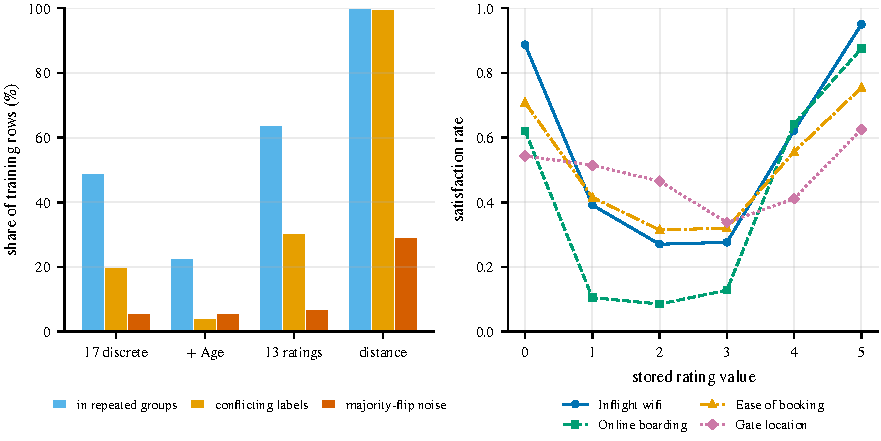
\includegraphics[width=\linewidth]{figures/fig_audit.pdf}
\caption{Left: share of training rows whose discrete signature repeats, whose labels conflict
inside such groups, and the fraction of labels that a majority vote would flip, for four
grouping keys. Right: satisfaction rate as a function of the stored rating. A stored~0 is a
``not applicable'' code, not a low score: Wi-Fi rating~0 is the \emph{most} satisfied group
(88.7\%), and every curve is non-monotone.}
\label{fig:audit}
\end{figure}

\subsection{The generator preserved distances and destroyed delays}
\label{sec:regen}
The competition data derive from a public survey of 129{,}880 passengers. Matching the two
files on the feature schema gives a precise picture of what the generator kept and what it
lost. The support of \texttt{Flight Distance} was copied almost verbatim: only 3 of the
3{,}474 distances in the training set do not occur in the survey, covering 0.0006\% of rows.
More importantly, the per-distance satisfaction rate survived: across the 2{,}243 distances
with at least 30 synthetic rows, the correlation between the synthetic and the original rate is
0.899 (Spearman 0.896), and the original rate alone scores \auc{} $=0.731$ on the synthetic
data. This is why a target encoding of the exact distance is the single most valuable feature
(Section~\ref{sec:single}): with the default \texttt{max\_bin}=255 the tree model can only
approximate 3{,}474 per-distance rates with 255 bins.

The delay columns were destroyed. In the survey, departure delay has mean 14.71 minutes and
99th percentile 180; in the synthetic data the mean is 1.18 and the 99th percentile 30, with
a point-biserial correlation of $-0.036$ against the label ($-0.051$ in the survey). Any
delay-based feature therefore has nothing to work with, which matches the negative ablation
in Figure~\ref{fig:ablation}.

\subsection{Rating zero is a missing-value code}
\label{sec:zero}
Figure~\ref{fig:audit}b shows the conditional satisfaction rate for each value of four ratings.
The curve is not monotone, and it is not noise: a Wi-Fi rating of 0 is reported by 1.87\% of
passengers and 88.7\% of them are satisfied, while a rating of 1 corresponds to 39.1\%.
Online boarding has the same shape (62.0\% at 0, 10.5\% at 1, 87.5\% at 5). Two consequences
follow. Trees can exploit the pattern with a single split at $\leq 0$, so no ``is-zero''
feature is needed (we tested it: $-0.04$ \dlt{}). A linear model, however, must see the ratings
one-hot encoded: on the same folds, logistic regression scores 0.9216 with the ratings treated
as numbers and 0.9486 with one-hot ratings, a difference of $2.7\times10^{-2}$.

\subsection{No exploitable row-level leak}
\label{sec:leak}
Because the data are synthetic, one may hope to recover the generating rows of the original
survey and inherit their labels. 27.07\% of training rows share their full 17-column signature
with a survey row, and for those rows the survey label agrees with the synthetic label 93.6\%
of the time --- but the model is better than the source: on the matched rows its \auc{} is
0.9428 while the survey label scores 0.9028, and a 50/50 blend of the two drops the overall
out-of-fold score from 0.9605 to 0.9592. We also tested for order leaks: consecutive identifiers
never share a signature, the autocorrelation of the label is smaller than $10^{-3}$, and the
mean absolute difference of flight distance between adjacent rows is 1{,}017 against 1{,}019 for
random pairs. The row order carries no information.

\section{Evaluation protocol}
\label{sec:protocol}

\subsection{Folds, fits and cross-fitting}
All experiments use five stratified folds (seed 42) and, for confirmations, a second five-fold
split (seed 2026). Every learned transform --- medians for imputation, category vocabularies,
target encodings, word frequencies --- is fitted on the training part of the fold only. Target
statistics use \texttt{sklearn}'s \texttt{TargetEncoder} with \texttt{smooth='auto'} and an inner
five-fold cross-fit \citep{miccibarreca2001}, so a training row never sees its own label
through the encoding. Each fold yields out-of-fold probabilities; the headline number is the
mean of the five fold scores, and we also report the pooled out-of-fold \auc{}.

\subsection{Paired inference and the noise floor}
Two models scored on the same out-of-fold predictions are highly correlated, so the relevant
uncertainty is the standard error of their \emph{difference}. We use the DeLong placement-value
covariance \citep{delong1988}, which gives a closed form for
$\mathrm{SE}[\widehat{\mathrm{AUC}}_a-\widehat{\mathrm{AUC}}_b]$. On this data set the single-model
\auc{} has a standard error of about $8.5\times10^{-4}$, but the paired standard error of a
difference is only \dlt{2.2}--\dlt{2.7}. That number is the resolution of the whole study:
\emph{any change below $2.2\times10^{-4}$ cross-validated is indistinguishable from noise on one
five-fold split.} For comparison, retraining the same model with a different seed moves the
five-fold mean by \dlt{0.9} and the public score by \dlt{1.2}, which agrees.

\subsection{An adoption rule fixed before the experiment}
To avoid the usual drift of adopting whatever looks better, the rule is written into the code
before a candidate is trained: a candidate is adopted only if it improves the mean fold \auc{}
on both splits with at least four of five folds ahead, and the paired test on the primary split
returns $p<0.10$. The threshold is deliberately looser than the $p<0.05$ used for scientific
claims, because ensembling is a variance-reduction mechanism with a known sign; but it still
blocks the $10^{-5}$-scale changes. When the owner of the repository overrode the rule, the
override was recorded in the model-selection file together with the observed $p$, which keeps
the audit trail honest.

\section{The single-model ceiling}
\label{sec:single}

\subsection{Baselines}
Table~\ref{tab:baselines} reports the five baselines under the protocol above. The gradient
boosting models are close to each other (LightGBM \citep{lightgbm_docs} 0.9586,
XGBoost \citep{chen2016} 0.9585, CatBoost \citep{prokhorenkova2018} 0.9577 with its default 500
iterations), the linear model is far behind on numeric ratings (0.9216), and the constant
predictor defines the trivial floor.

\begin{table}[t]
\centering
\small
\caption{Baselines on the five fixed folds. Mean and population standard deviation of the fold
\auc{}, pooled out-of-fold \auc{} and log loss.}
\label{tab:baselines}
\begin{tabular}{lcccc}
\toprule
Model & mean fold \auc{} & std & OOF \auc{} & OOF log loss\\
\midrule
Constant prior            & 0.50000 & 0.00000 & 0.50000 & 0.68677\\
Logistic regression       & 0.92156 & 0.00043 & 0.92156 & 0.34424\\
CatBoost (500 it.)        & 0.95770 & 0.00066 & 0.95770 & 0.23057\\
XGBoost (500 it.)         & 0.95846 & 0.00061 & 0.95845 & 0.22842\\
LightGBM (500 it.)        & 0.95862 & 0.00059 & 0.95861 & 0.22789\\
\bottomrule
\end{tabular}
\end{table}

\subsection{What moved the single model, and what did not}
The ladder in Figure~\ref{fig:progress}a starts at 0.9586 for a raw LightGBM. Adding five
crossed categorical features (travel$\times$cabin, cabin$\times$boarding, \ldots) gives
\dlt{1.6} and 16 Optuna trials \dlt{2.4}; both are inside or at the edge of the noise band. The
first large step is the cross-fitted target statistics of the flight-distance keys:
$+13.5$ \dlt{} ($p=5\times10^{-4}$), which is the only single change in the whole study that
clears the noise floor by a wide margin. Smoothing those encodings with the empirical-Bayes
default adds \dlt{1.65} ($p=0.46$); we kept it because it also minimised the tuned objective,
but we do not claim it is a real improvement.

Capacity is saturated. Doubling the number of trees (500 $\to$ 1{,}000) costs \dlt{0.9};
reducing the leaves from 63 to 31 costs \dlt{2.1}; a 127-leaf model at learning rate 0.03
peaks at 500 trees and then degrades; a 255-leaf model at rate 0.02 degrades monotonically
(0.9597 at 500 trees down to 0.9585 at 3{,}000). The validation curve flattens at about 400
trees. The sixteen Optuna trials that produced the adopted configuration are spread over
$9.5\times10^{-4}$, and the top two trials differ by $10^{-5}$ --- a ranking of noise.

\begin{figure}[t]
\centering
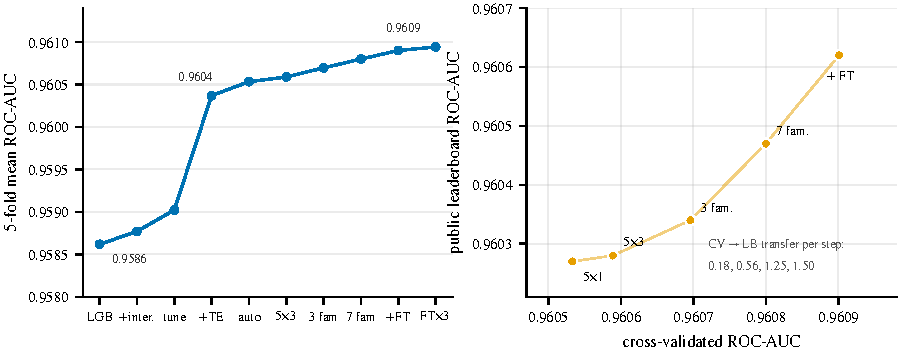
\includegraphics[width=\linewidth]{figures/fig_progress.pdf}
\caption{Left: five-fold mean \auc{} along the modelling path. Right: the same models on the
public leaderboard. Each submitted model sits about \dlt{3} below its cross-validated score ---
the constant offset between the two readings --- but the \emph{per-step} transfer grows with
the diversity of the ensemble.}
\label{fig:progress}
\end{figure}

\section{Model families and blending}
\label{sec:families}

Once single-model capacity is exhausted, the only remaining mechanism with a plausible sign is
to combine models whose errors are not the same. We therefore trained nine members under the
same folds and transforms: LightGBM with the adopted target statistics, four other boosted
configurations (XGBoost, CatBoost with 2{,}500 GPU iterations and native categorical handling,
LightGBM with linear leaves, LightGBM with DART dropout), two multilayer perceptrons (one on the
raw frame with embeddings, one on the 33 encoded numeric features), an FT-Transformer
\citep{gorishniy2021}, and --- as a deliberately different information source --- a model trained
only on the 129{,}880 original survey rows.

\paragraph{The FT-Transformer.} Each feature becomes a token: an embedding for each of the 17
discrete fields (including the 3{,}474-level flight distance), a linear projection for each of
the four continuous fields, and a two-level embedding for the arrival-delay missing flag.
A learnable class token is prepended and three pre-normalised transformer blocks
($d=64$, four heads, FFN width 128, dropout 0.1) process the 23 tokens; a linear head on the
class token outputs the logit. Training uses AdamW and a one-cycle schedule for 20 epochs at
batch 4{,}096, which costs 97 seconds per fold on a laptop GPU --- cheap enough for five folds
in eight minutes.

\paragraph{Weights follow decorrelation, not strength.} Figure~\ref{fig:members} shows the two
quantities that matter for a member: its own score and the correlation of its residuals with
the LightGBM member. Fitting non-negative weights that sum to one on the logits
(Section~\ref{sec:stacking}) gives the lower panel. The best single model, LightGBM, ends up
with weight 0.012, while CatBoost (0.207), \texttt{linear\_tree} (0.179), XGBoost (0.155) and
the FT-Transformer (0.249) carry the ensemble. The FT-Transformer is the clearest case: it is
$2.0\times10^{-3}$ weaker than LightGBM alone and yet takes the largest weight, because it is
the most different strong member.

\begin{figure}[t]
\centering
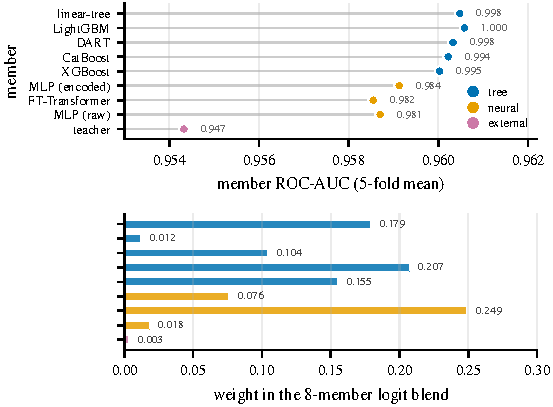
\includegraphics[width=0.68\linewidth]{figures/fig_members.pdf}
\caption{Members of the eight-family blend. Top: five-fold mean \auc{} with the residual
correlation against LightGBM printed next to each point. Bottom: weight fitted on the logits.
Strength and weight are almost independent: the two MLPs and the FT-Transformer absorb the
weight that the boosted trees cannot supply.}
\label{fig:members}
\end{figure}

Table~\ref{tab:blends} traces the ensemble. Three families (LightGBM, XGBoost, MLP) add
\dlt{1.07} over the multi-seed single model; five more members \dlt{1.0}; the FT-Transformer
another \dlt{1.0}. Each of these steps is at the noise floor on its own, but they are
\emph{cumulative} and each is confirmed by the leaderboard, which is the point of
Section~\ref{sec:lb}.

\begin{table}[t]
\centering
\small
\caption{Ensemble ladder. ``Public'' is the leaderboard score of the submitted file; the
transfer column is $\Delta$public$/\Delta$CV for that step.}
\label{tab:blends}
\begin{tabular}{lcccccc}
\toprule
Configuration & CV & OOF & public & rank & $\Delta$CV (\dlt{}) & transfer\\
\midrule
5 folds $\times$ 1 seed                & 0.960533 & 0.960526 & 0.96027 & 1331/2977 & --- & ---\\
5 folds $\times$ 3 seeds               & 0.960589 & 0.960580 & 0.96028 & 1340/2991 & $+0.55$ & 0.18\\
3 families (LGB+XGB+MLP)               & 0.960696 & 0.960688 & 0.96034 & 1307/3000 & $+1.07$ & 0.56\\
7 families                             & 0.960800 & 0.960793 & 0.96047 & 1254/3013 & $+1.04$ & 1.25\\
8 families ($+$FT-Transformer)          & 0.960901 & 0.960891 & \textbf{0.96062} & \textbf{1204/3061} & $+1.00$ & 1.50\\
8 families ($+$FT$\times$3 seeds)      & \textbf{0.960942} & 0.960932 & 0.96061 & --- & $+0.42$ & $-0.02$\\
\bottomrule
\end{tabular}
\end{table}



\section{What does not work}
\label{sec:rejected}

Figure~\ref{fig:ablation} collects the interventions that attribute to a single change, with
their measured effect. The lower half of the list is as informative as the upper half.

\paragraph{Variance control.} Averaging three seeds per fold buys \dlt{0.55} in CV and
\dlt{0.1} on the leaderboard. Ten folds instead of five buys \dlt{0.14} cross-validated: the
probe in Table~\ref{tab:protocol} shows that training each model on 72\% instead of 64\% of the
data helps, but the extra averaging over ten models cancels it (10 folds $\times$ 3 seeds:
0.961355; 5 folds $\times$ 3 seeds: 0.961356 on the same probe split). Strengthening the best
member behaves the same way: three seeds lift the FT-Transformer from 0.958548 to 0.959258 and
the blend from 0.960901 to 0.960942, yet the public score moves from 0.96062 to 0.96061.

\begin{table}[t]
\centering
\small
\caption{Protocol probe on a fixed 20\% split (139{,}927 rows): the dev part is re-split into
$k$ folds, each model is trained on $k-1$ of them and the predictions are averaged before
scoring. ``Train fraction'' is relative to the full training file.}
\label{tab:protocol}
\begin{tabular}{lcccc}
\toprule
Configuration & train fraction & probe \auc{} & $\Delta$ (\dlt{}) & time\\
\midrule
5 folds $\times$ 1 seed   & 0.64 & 0.961305 & --- & 47 s\\
5 folds $\times$ 3 seeds  & 0.64 & 0.961356 & $+0.55$ & 96 s\\
10 folds $\times$ 1 seed  & 0.72 & 0.961319 & $+0.14$ & 106 s\\
10 folds $\times$ 3 seeds & 0.72 & 0.961355 & $+0.50$ & 211 s\\
\bottomrule
\end{tabular}
\end{table}

\paragraph{Stacking.}
\label{sec:stacking}
We tried five meta-learners on the member logits, all cross-fitted (fit on four folds, predict
the held-out one): logistic regression with four values of $C$, a LightGBM meta-model on the
seven logits, the same plus member-disagreement features, the same plus the 21 raw features
(conditional stacking), and one weight vector per cabin$\times$travel segment. None of them
beats the fixed mean-weight blend (Table~\ref{tab:stacking}). The reason is visible in
Figure~\ref{fig:members}: with residual correlations between 0.977 and 1.000 the meta-model has
nothing to learn except a global reweighting, and the fitted weights already do that. A
meta-model can only pay when the members are both strong and genuinely different.

\begin{table}[t]
\centering
\small
\caption{Cross-fitted stacking against the fixed-weight blend (0.960800). ``$z$'' is the paired
DeLong statistic; every value is statistically indistinguishable from zero.}
\label{tab:stacking}
\begin{tabular}{lcccc}
\toprule
Meta-learner & fold mean & $\Delta$ (\dlt{}) & folds ahead & $z$\\
\midrule
Logistic on logits ($C=0.01$--$10$)   & 0.960797 & $-0.04$ & 1/5 & $-0.6$\\
LightGBM on 7 logits                  & 0.960799 & $-0.01$ & 3/5 & $-0.3$\\
LightGBM on logits $+$ spread         & 0.960826 & $+0.26$ & 4/5 & $-0.2$\\
LightGBM on logits $+$ raw features   & 0.960811 & $+0.11$ & 3/5 & $-0.2$\\
Per-segment weight vectors (6)        & 0.960810 & $+0.09$ & 3/5 & $+0.1$\\
\bottomrule
\end{tabular}
\end{table}

\paragraph{Feature-side variants.} Multi-view auxiliary features (three LightGBMs trained on
feature subsets, their cross-fitted logits appended) give \dlt{0.57} at $p=0.81$ and three of
five folds: rejected. Pseudo-labelling the 6.6\% of test rows the blend is confident about
produces a member at 0.960549 with residual correlation 0.9994 --- worse than the plain
LightGBM it was meant to help. A target encoding of the full 17-column signature, extra
distance-segment encodings and \texttt{max\_bin}$=4095$ are all at or below zero.

\paragraph{Weak but different is not enough.} The teacher trained only on the original survey is
the most decorrelated member we found (residual correlation 0.947, against 0.981 for the best
MLP) and it is worthless: at 0.954326 its fitted weight is 0.003. Contribution requires
\emph{both} properties --- a member needs to be within about $2\times10^{-3}$ of the leader and
have a residual correlation below roughly 0.99. Finally, PyTabKit's RealMLP with default
hyper-parameters \citep{holzmuller2024} trained for 30 epochs costs 6.9 minutes per fold and
reaches only 0.958281, so we did not include it; the published recipe relies on an ensemble of
many seeds, which is the family-level move we already exploit through the FT-Transformer.

\begin{figure}[t]
\centering
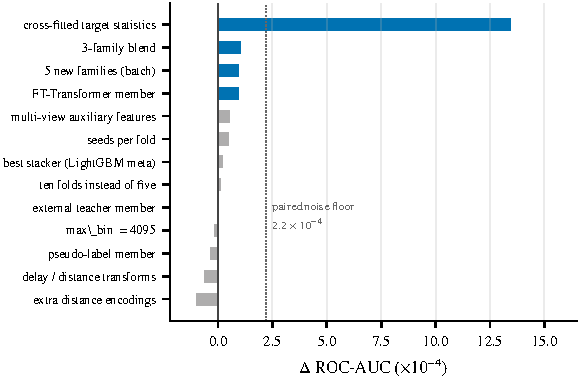
\includegraphics[width=0.68\linewidth]{figures/fig_ablation.pdf}
\caption{Every intervention measured against the same reference, in units of \dlt{}.
Blue: adopted. Grey: measured and rejected. The dotted line is the paired noise floor
(\dlt{2.2}); everything to its left is indistinguishable from retraining with another seed.}
\label{fig:ablation}
\end{figure}

\section{Reading the leaderboard}
\label{sec:lb}

\subsection{The ladder, and why CV under-predicts the gain}
Table~\ref{tab:blends} and Figure~\ref{fig:progress}b tell one coherent story. Every model sits
about \dlt{3} below its cross-validated score --- the offset is remarkably stable
($-2.6$, $-3.1$, $-3.6$ \dlt{} across versions), which is what an exchangeable split predicts.
What changes is the \emph{slope}: the same $+1.0$ \dlt{} of cross-validated improvement is worth
$+0.1$ \dlt{} when it comes from seed averaging, $+0.6$ when it comes from a three-family blend,
$+1.3$ when it comes from seven families and $+1.5$ when the FT-Transformer joins. Averaging
different \emph{functions} generalises better than averaging one function many times, and the
public split (299{,}844 rows) sees that more clearly than five validation folds of 140{,}000
rows each.

The counter-example is equally instructive: three-seeded FT-Transformer is the best
cross-validated model we built (0.960942) but scored 0.96061, one $10^{-5}$ below its
single-seeded sibling. We therefore kept the leaderboard-best artifact and recorded both
numbers in the model-selection file. Reporting the CV-best number while shipping the LB-best
file would have been the easy way to make this section look better than it is.

\subsection{What the leaderboard's shape implies}
Figure~\ref{fig:rank} converts the remaining gap into effort: near our band roughly 50 places
cost $10^{-4}$ of \auc{}, so the 1.1 \dlt{} that separate us from the top decile (0.96192) is
about 550 places. Two further observations from the snapshot of 3{,}061 teams help calibrate
what such a jump would require.

First, the board is dominated by ties. Of 3{,}013 teams in an earlier snapshot only 749 distinct
scores exist, and 130 teams share the single value 0.96213 (ranks 21--150). A 130-way tie at
five decimals is not 130 independent discoveries; it is the signature of a shared artifact ---
published out-of-fold predictions and frozen stacks, which are explicitly distributed in this
competition. Second, submission counts increase with rank: the median top-10 team has made 47
submissions against 4 for the field, and the top two have made 178 and 150. Because the public
board records a team's best public submission, part of the visible gap is selection, not skill;
the private split will settle it.

Finally, the two leaders are outliers in a way that stacking arithmetic does not explain:
$+0.64$ \dlt{} above rank 2 and $+1.04$ \dlt{} above rank 3, whereas ranks 3--10 span only
$0.32$ \dlt{}. We could not identify the mechanism from public material, and we ruled out the
leak candidates we could test (Section~\ref{sec:leak}).

\begin{figure}[t]
\centering
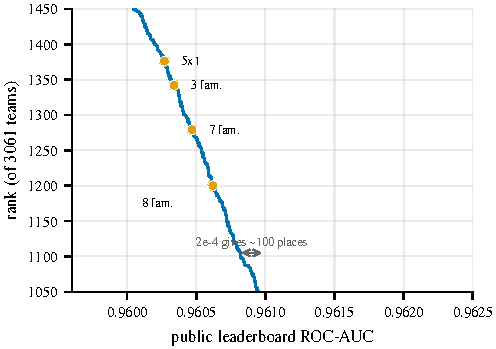
\includegraphics[width=0.68\linewidth]{figures/fig_rank.pdf}
\caption{Public leaderboard rank against score, zoomed on the band around our submissions.
Near this score, \dlt{2} of \auc{} buys roughly one hundred places; the top decile is
1.1 \dlt{} away.}
\label{fig:rank}
\end{figure}

\section{Discussion and limitations}

\paragraph{A rule of thumb.} Across the interventions we measured, the outcome is summarised by
one sentence: \emph{changes that alter the hypothesis class transfer to unseen data; changes that
reduce the variance of a fixed hypothesis class mostly do not.} The target encoding of the
distance is the extreme case of the first kind ($+13.5$ \dlt{}, transfer $\approx1$), a new
architecture family is a milder version of it ($+1.0$ \dlt{}, transfer 1.5), and seed
averaging, fold count, stackers and pseudo-labels belong to the second kind. The practical
consequence is a budget rule: if a change costs more than an hour and is expected to buy less
than \dlt{3} in CV, it will not be visible on a board whose granularity is $10^{-4}$.

\paragraph{The remaining gap is a budget, not a trick.} The top decile needs 1.1 \dlt{} more.
At $2$--$5$ \dlt{} per qualifying member (strong and residual-correlated below 0.99), that is
20--50 additional members --- consistent with the hundreds of members that public stacks
combine. We did not pursue the shared-OOF route, which is the only way to reach that scale
within a competition, because it cannot be reproduced from a repository that does not own the
other teams' predictions.

\paragraph{Limitations.} (i) One competition, one metric, one month; the transfer rates are
specific to a 300k-row public split and to a synthetic generator whose noise is unusually high.
(ii) The public board is a moving target: team counts changed from 2{,}977 to 3{,}061 during the
study, and ties are resolved by submission time, so rank changes smaller than about 20 places
are not meaningful. (iii) Part of the top of the board is selection over many submissions and
cannot be attributed to modelling. (iv) Our adoption gate was overridden twice by the
repository owner; both overrides are recorded with the observed $p$-values rather than hidden.
(v) The study uses a single GPU and a single machine; timings are not comparable across
hardware.

\section{Reproducibility}
Every number in this paper comes from a command in the repository. Folds and their hashes are
stored with the preprocessors; model-selection files record weights, seeds, cross-validated
scores, confirmation splits and the adoption gate.

\begin{center}
\small
\begin{tabular}{ll}
\toprule
Stage & Command\\
\midrule
Preprocess and fix folds        & \texttt{python main.py preprocess} ; \texttt{main.py cv}\\
Baselines and ablations         & \texttt{main.py baseline} ; \texttt{main.py features}\\
Target statistics               & \texttt{main.py targetstats} ; \texttt{main.py explore}\\
Hyper-parameter search          & \texttt{main.py tune --trials 16}\\
Multi-seed final model          & \texttt{main.py final --seeds 42 1042 2042}\\
Multi-family blend              & \texttt{main.py multimodel --weights 0.8 0.1 0.1}\\
Data audit                      & \texttt{python analysis/audit.py}\\
Tests                           & \texttt{python -m unittest discover -s tests}\\
\bottomrule
\end{tabular}
\end{center}

The FT-Transformer member, the stacking study and the multi-family weight search were run as
recorded experiment scripts; their outputs (out-of-fold predictions, test predictions, weights,
paired statistics) are the inputs of the tables above. The 34 unit tests of the repository
cover the leakage guarantees on which the protocol relies: per-fold fitting, unknown categories,
probability bounds and OOF alignment.

\section*{Acknowledgments}
An AI research assistant helped orchestrate the experiments and prepare the manuscript. Every
number in the tables above is reproducible from the recorded scripts, and every experiment was
retained whether or not it succeeded.

\bibliographystyle{plainnat}
\bibliography{references}


\end{document}

